\chapter{Finding Unsatisfiable Cores Extraction for a Set of Polynomials using the Gr\"obner Basis Algorithm}
\label{ch:UNSAT}
Besides elimination ideal based abstraction, Gr\"obner basis can also be applied to a vast field
about other techniques in formal verification. Satisfiability (SAT) problem is the basis of modern 
computation theories, as well as the origin of most formal verification problem. 
In this chapter, we will discuss a sort of problems branching out from SAT. They are about a situation 
when SAT problems give negative answer, which are called unsatisfiability (UNSAT) problems. Within 
a set of constrains (e.g. clauses, formulas or polynomials) which is unsatisfiable, sometimes 
it is worthy to explore a smaller subset (core) that keeps UNSAT. From the execution of GB algorithm, 
an auxiliary structure can be obtained to help UNSAT core extraction. This chapter will introduce the 
details about the motivation, mechanism and implementation. 

\section{Motivation}
\subsection{Exploiting UNSAT cores for abstraction refinement}
By exploring previous work, we learn that most state-of-art abstraction refinement techniques require 
information mining from UNSAT proofs of intermediate abstractions. 
Here we use an abstraction refinement algorithm from \cite{zhang2005design} to explain that how an UNSAT proof is
utilized in such techniques.

\IncMargin{1em}
\begin{algorithm}[H]
\SetAlgoNoLine
\LinesNumbered
	\KwIn{$M$ -- original machine, $p$ -- property to check, $k$ -- \# of steps in $k$-BMC}
	\KwOut{If $p$ is violated, return error trace; otherwise $p$ is valid on $M$}
  $k = $ InitValue\;
  
  \eIf{$k$-BMC$(M,p,k)$ is \textbf{SAT}}
  {
	\Return{``Found error trace"}
  }
  {
	Extract UNSAT proof $\mathcal P$ of $k$-BMC\;
	$M' = $ \textit{ABSTRACT}$(M,\mathcal P)$\;
  }
  \eIf{MODEL-CHECK$(M',p)$ returns \textbf{PASS}}
  {
	\Return{``Passing property"}
  }
  {
	Increase bound $k$\;
	goto Line 2\;
  }
\caption {Abstraction refinement using $k$-BMC}\label{alg:absrefine}
\end{algorithm}
\DecMargin{1em}


\begin{figure}[hbt]
\centering{
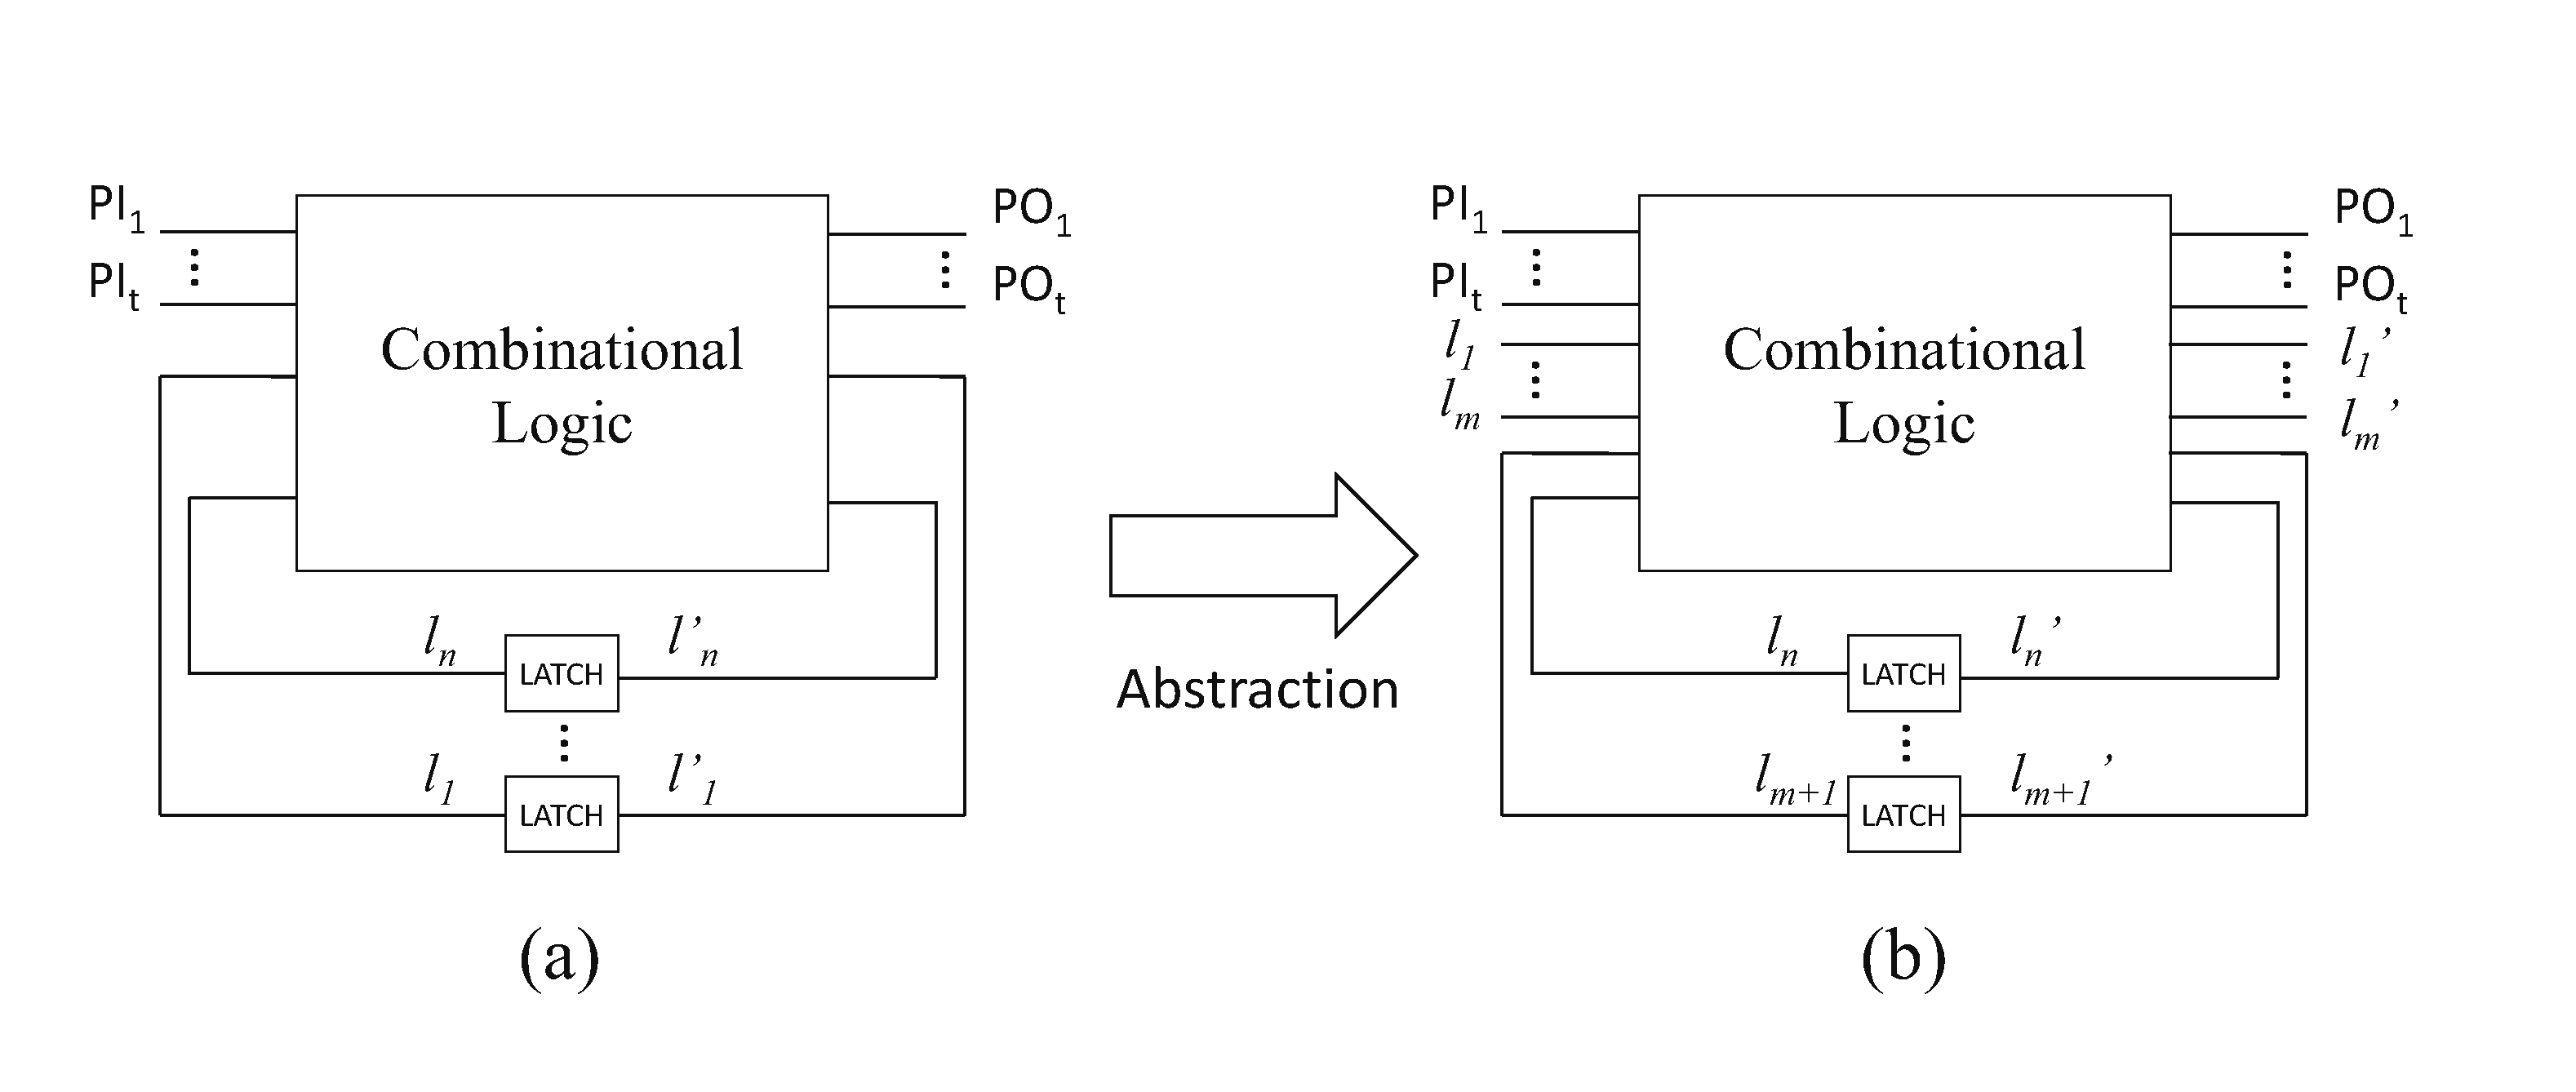
\includegraphics[width=5.5in]{newfig/refine.eps}
\caption{Abstraction by reducing latches}
\label{fig:refine}}
\end{figure}
Assume that we are given a sequential circuit with $n$ latches as shown in Fig.\ref{fig:refine}(a). 
This circuit can be modeled as a Mealy machine $M$ and the states $s$ can be explicitly encoded by bit-level latch variables 
$l_1,\dots,l_n$. Algorithm \ref{alg:absrefine} describes an approach to check if machine $M$ violates property $p$.
This algorithm relies on $k$-BMC technique, which works on the basis of CNF-SAT solving.
The $k$-BMC represents the initial states $I$, the transition relation $T$ and property $p$ as CNF formulas.

The first ``if-else" branch in Algorithm \ref{alg:absrefine} can be
explained as: we check if the conjunction of formulas 
$$I(s_0)\land \bigwedge_{i=0}^{k-1}T(s_i,s_{i+1}) \land \neg p$$
is $SAT$ or not, where $s_i$ denotes the set of reached states in $i$-th time-frame. If the result is
$SAT$, then a counterexample is found that violates property $p$. If the result is $UNSAT$, we cannot
assert that $p$ is satisfied for the original machine $M$ because we only unrolled $M$ for a given specific number of time-frames
without any fixpoint detected.
In this algorithm, we analyze the UNSAT core composed by a set of clauses whose conjunction is $UNSAT$.
If there are some latch variables not included in this UNSAT core (denoted by $L_{abs}$), then we can assert that the evaluations of 
these variables will not affect the unsatisfiability of original formula. Therefore, we can ignore them in the abstracted model.
In practice, we turn these latches into primary inputs/outputs as shown in Fig.\ref{fig:refine}(b) ($L_{abs} = \{l_1,\dots,l_m\}$).


The second ``if-else" branch means: if we do an ordinary model checking on the abstracted machine $M'$ and find no
error trace, we can assert that property $p$ also holds on the original machine $M$. The reason of this assertion is that
the abstracted states represented using abstracted latches cover the original states, which means $M'$ is an over-approximation
of $M$, such that $(M'\implies p) \implies (M\implies p)$. If we find a violation on abstracted machine, then this
abstracted model is not a suitable model to check $p$, so we have to increase the bound $k$ to find a finer abstraction.

It is clear that UNSAT cores play an important role in abstraction refinement approaches. In \cite{zhang2005design}
the UNSAT core is extracted using a conventional CNF-SAT solver, which will encounter the ``bit-blasting" problem
when the size of datapath (number of latches in Fig.\ref{fig:refine}) is very large. \textbf{Here we propose a totally new 
method based on Gr\"obner basis computation to extract UNSAT cores, and we believe it may become an efficient 
method according to the following observation based on our experience:}

% {\it Gr\"obner basis is more suitable for UNSAT problems because of following theorem:}
{\it While computing GB over finite fields is exponential in the number of variables, GB  computation 
is observed to be more efficient for UNSAT problems.} 
The reason is discussed as follows:
\begin{Theorem}
{\bf Weak Nullstellensatz:} Given ideal $J\subset \mathbb F[x_1,\dots,x_n]$, its variety over algebraic closure
of field $\mathbb F$ is empty if and only if its reduced Gr\"obner basis contains only one generator ``1".
$${\bf V}_{\overline{\mathbb F}}(J) = \emptyset \Longleftrightarrow reducedGB(J) = \{1\}$$
\end{Theorem}
It is well known that using Buchberger's algorithm and its variations to compute a GB has a very high
time complexity and is usually not practicable. One reason is that the size of GB may explode even if the term
ordering is carefully chosen. However if the reduced GB is 1, which means every term in the original polynomials
will be canceled, the degree of remainders when computing GB with Buchberger's algorithm will be limited. 
Thus the number of polynomials in non-reduced GB is much smaller than usual.
Instead of applying polynomial calculus to SAT solving, it may be more efficient to try it for UNSAT
problems.

\subsection{A Demonstration of Motivating Example}
One  important research topic about UNSAT problems is to identify UNSAT cores efficiently.
An UNSAT core in a CNF formula denotes a subset of clauses which is still unsatisfiable. Here
we re-define this concept in algebraic geometry:
\begin{Definition}
Assume a set of polynomials $F$ and its subset $F_s\subset F$. If ${\bf V}(\langle F\rangle) = {\bf V}
(\langle F_s\rangle) = \emptyset$, we call $F_s$ an {\bf UNSAT core} of $F$. Additionally, if
$F_s$ contains no other UNSAT core, we call it a {\bf minimal} UNSAT core.
\end{Definition}

We  conjecture that based on observation of Buchberger's algorithm's execution, an UNSAT core can be identified.
\begin{Proposition}
Buchberger's algorithm picks pairs of polynomials from a given set, computes their S-poly, then reduces this S-poly
with the given set of polynomials. If the remainder is non-zero,
it is added to the set of polynomials.
By tracking S-poly computations and multivariate divisions that lead to remainder 
1, we can obtain an UNSAT core. Moreover, we can identify a minimal UNSAT core with one-time
 execution of Buchberger's algorithm.
\end{Proposition}
\begin{Example}
A SAT problem is described with 8 CNF clauses:

\begin{minipage}[h]{0.3\textwidth}
\begin{align*}
&c_1: \bar{a}\lor\bar{b}\\
&c_2: a\lor\bar{b}\\
&c_3: \bar{a}\lor b\\
&c_4: a\lor b
\end{align*}
\end{minipage}
\begin{minipage}[h]{0.7\textwidth}
\begin{align*}
&c_5: x\lor y\\
&c_6: y\lor z\\
&c_7: b\lor \neg y\\
&c_8: a\lor x\lor \neg z
\end{align*}
\end{minipage}

% \begin{align*}
% &\bar{a}\lor\bar{b}\\
% &a\lor\bar{b}\\
% &\bar{a}\lor b\\
% &a\lor b\\
% &x\lor y\\
% &y\lor z\\
% &b\lor \neg y\\
% &a\lor x\lor \neg z
% \end{align*}
Using Boolean to polynomial mappings given in Table \ref{tab:booltof4}, we can transform them to a set of
polynomials $F$ over ring $\mathbb F_2[a,b,x,y,z]$:

\begin{minipage}[h]{0.4\textwidth}
\begin{align*}
&f_1:ab\\
&f_2:ab+a\\
&f_3:ab+b\\
&f_4:ab+a+b+1
\end{align*}
\end{minipage}
\begin{minipage}[h]{0.6\textwidth}
\begin{align*}
&f_5:xy+y+x+1\\
&f_6:yz+y+z+1\\
&f_7:by+y\\
&f_8:axz+az+xz+z
\end{align*}
\end{minipage}
% \begin{align*}
% &f_1:ab\\
% &f_2:ab+a\\
% &f_3:ab+b\\
% &f_4:ab+a+b+1\\
% &f_5:xy+y+x+1\\
% &f_6:yz+y+z+1\\
% &f_7:by+y\\
% &f_8:axz+az+xz+z
% \end{align*}
We compute its GB using Buchberger's algorithm with lexicographic term ordering $a>b>x>y>z$.
Since this problem is UNSAT, we will stop when ``1" is added to GB.
\begin{enumerate}
\item First we compute $Spoly(f_1,f_2)\xrightarrow{F}_{+} r_1$, remainder $r_1$ equals to $a$;
\item Update $F=F\cup r_1$;
\item Next we compute $Spoly(f_1,f_3)\xrightarrow{F}_{+} r_2$, remainder $r_2$ equals to $b$;
\item Update $F=F\cup r_2$;
\item We can use a directed acyclic graph (DAG) to represent the process to get $r_1,r_2$, as Fig.\ref{fig:UNSAT}(a) shows;
\item Then we compute $Spoly(f_1,f_4) = s_3= a+b+1$, obviously $a+b+1$ can be reduced (multivariate divided) by
$r_1$ , the intermediate remainder $r_3 = b+1$. It can be immediately divided by $r_2$, and the remainder is ``1", we
terminate the Buchberger's algorithm;
\item We draw a DAG depicting the process through which we obtain remainder ``1" as shown in Fig.\ref{fig:UNSAT}(b). 
From leaf ``1" we backtrace the graph to roots $f_1,f_2,f_3,f_4$. They constitute an UNSAT core for this problem
as these polynomials are the ``causes" of unsatisfiability of original set of clauses.
\end{enumerate}
\end{Example}
\begin{figure}[hbt]
\centering{
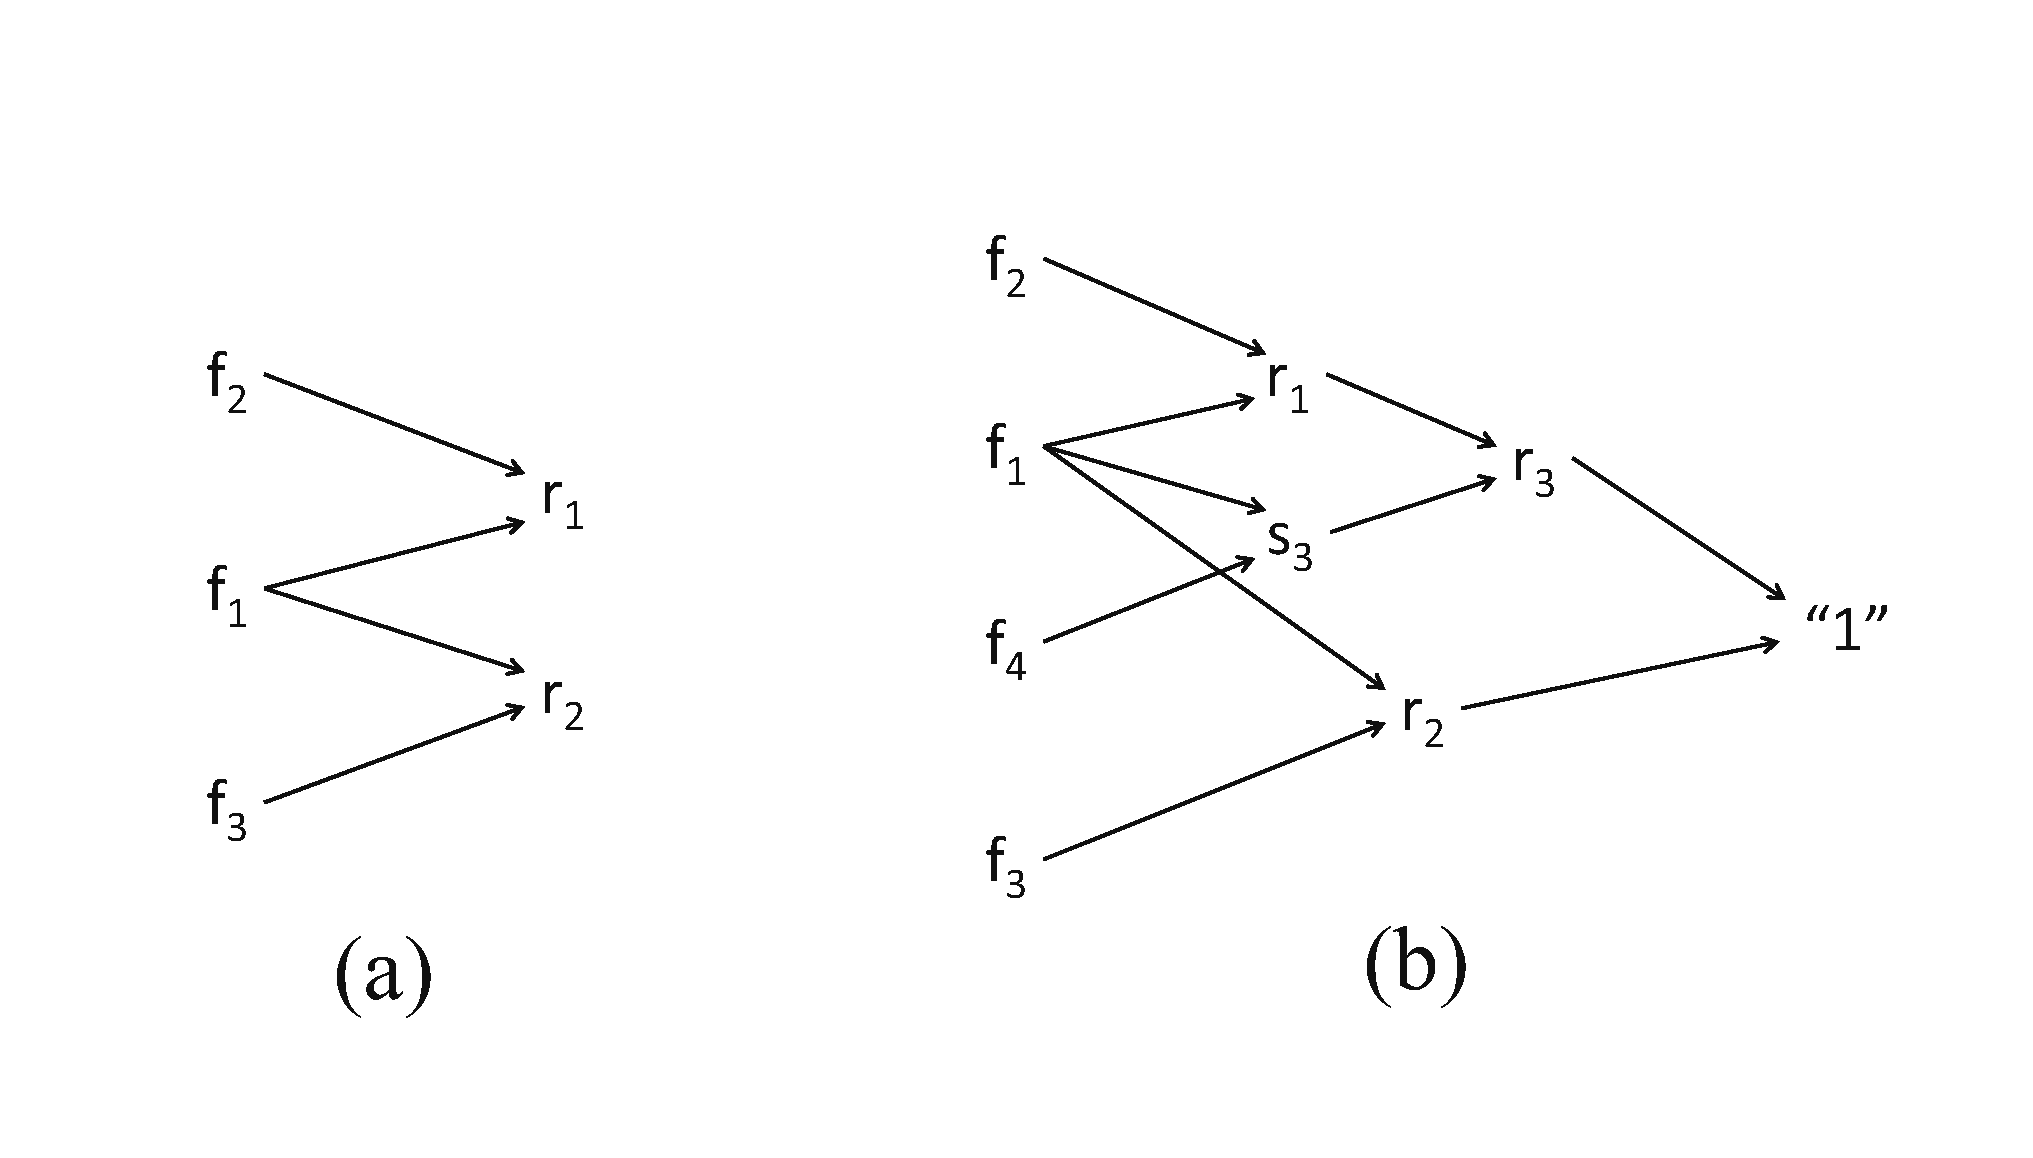
\includegraphics[width=\textwidth]{newfig/UNSAT.eps}
\caption{DAG representing Spoly computations and multivariate divisions}
\label{fig:UNSAT}}
\end{figure}
% We conclude our approach as follows: i) Keep track of all $Spoly(f_i,
% f_j)\xrightarrow{f_1, \dots, f_s}_+ r$; ii) mark $f_i, f_j$ if $r\neq
% 0$; iii) Mark those $f_l$'s that have leading terms that cancel
% monomial terms in $Spoly(f_i, f_j)$; iv) Build a DAG recording all reductions including Spoly computations
% and multivariate divisions; v) Once $1\in J$ is
% detected, traverse the graph to identify all the marked polynomials that were
% used in obtaining this unit element. These polynomials constitute the
% core.

We conclude our approach as a conjecture algorithm (Algorithm \ref{alg:UNSAT}). 

\begin{algorithm}[hbt]
\SetAlgoNoLine
	\KwIn{A set of polynomials $F = \{f_1,f_2,\dots,f_s\}$}
	\KwOut{An UNSAT core $\{f_{m_1},f_{m_2},\dots,f_{m_t}\}$}
\Repeat{$r_l == 1$}
{
	Pick a pair $f_i,f_j\in F$ that has never been computed S-poly\;
	\If{$Spoly(f_i,f_j)\xrightarrow{F}_+ r_l \neq 0$}
	{
		$F = F\cup r_l$\;
		Create a DAG $G_l$ with $f_i,f_j$ as roots, $r_l$ as leaf, recording the S-poly, all intermediate remainders and $f_k\in F$ that cancel monomial terms in the S-poly\;
	}
}
Backward traverse the DAG for remainder ``1", replace $r_l$ with corresponding DAG $G_l$\;
\Return{All roots}
\caption {Extract UNSAT core using a variation of Buchberger's algorithm}\label{alg:UNSAT}
\end{algorithm}

\section{Formalize the Buchberger's Algorithm based UNSAT Core Identification}
\label{sec:core}

\textbf{Problem: }
Let $F = \{f_1, \dots f_s\}$ be a set of multivariate polynomials in
the ring $R = \F[x_1,\dots,x_d]$ that generate ideal $J = \langle
f_1,\dots,f_s\rangle \subset R$. Suppose that it is known that $V(J) =
\emptyset$, or it is determined to be so by applying the Gr\"obner
basis algorithm. Identify a subset of polynomials $F_c \subseteq F,
J_c = \langle F_c \rangle$, such that $V(J_c) = \emptyset$
too. Borrowing the terminology from the Boolean SAT domain, we
call $F_c$ the infeasible core or the unsat core of $F$. 

%% Any set of polynomials $F$ with empty variety is an unsat core in
%% itself. There may be more than one unsat cores in $F$, some
%% polynomials may be common to multiple cores (i.e. the
%% cores may be non-disjoint), and these cores may have
%% different cardinalities $|F_c|$. The unsat core problems
%% are therefore further classified as: 
%% \bi
%% \item Identify a {\it minimum} core, i.e. a core of minimum
%%   cardinality. 
%% \item Identify a {\it minimal} core. An unsat core $F_{c}$ is minimal
%%   with respect to the property that while the variety of $F_{c}$ is
%%   empty, the variety of {\it any} subset of $F_c$ is {\it non-empty},
%%   i.e. $V( F_{c} - \{f_i\} ) \neq \emptyset$ for any $f_i \in
%%   F_c$. 
%% \item Identify any unsat core disregarding minimality; i.e. find any
%%   subset $F_c$ of $F$.
%% \ei

%% Let us first consider the problem of finding any $F_c \subset F$,
%% disregarding minimality. 
It is not hard to motivate that an unsat core should be identifiable
using the Gr\"obner basis algorithm: Assume that $F_c=F-\{f_j\}$. If
$GB(F) = GB(F_c) = \{1\}$, then it implies that $f_j$ is a member of
the ideal generated by $(F - \{f_j\})$, i.e. $f_j \in \langle F -
\{f_j\}\rangle$. Thus $f_j$ can be composed of the other
polynomials of $F_c$, so $f_j$ is  not a part of the unsat core, and
it can be safely discarded from $F_c$. This can be identified by means
of the GB algorithm for this ideal membership test.% (Def. \ref{def:gb}(ii)).  

A n\"aive way (and inefficient way) to identify {\it a minimal core}
using the GB computation is as follows:
select a polynomial $f_i$ and see if $V(F_c - \{f_i\}) = \emptyset$
(i.e. if reduced $GB(F_c - \{f_i\}) = \{1\}$). If so, discard $f_i$
from the core; otherwise retain $f_i$ in $F_c$. Select a different
$f_i$ and continue until all polynomials $f_i$ are visited for
inclusion in $F_c$. This approach will produce a minimal core, as we
would have tested each polynomial $f_i$ for inclusion in the
core. This requires $O(|F|)$ calls to the GB engine, which is really
impractical.   

\subsection{The Refutation Tree of the GB Algorithm: Find $F_c$ from $F$}

We investigate if it is possible to identify a core by analyzing the
$Spoly(f_i,f_j)\xrightarrow{F}_+ g_{ij}$ reductions in Buchberger's
algorithm. Since $F$ is itself an unsat core, 
definitely {\it there exists  
a sequence of Spoly reductions in Buchberger's algorithm where
$Spoly(f_i, f_j) \xrightarrow{F}_+ 1$ is achieved.} Moreover, 
polynomial reduction algorithms can be suitably modified to record
which polynomials from $F$ are used in the division leading to
$Spoly(f_i,f_j)\xrightarrow{F}_+1$. This suggests that 
we should be able to identify a core by recording
the {\it data} generated by Buchberger's algorithm --- namely, the
critical pairs($f_i,f_j$) used in the Spoly computations,
and the polynomials from $F$ used to cancel terms in the reduction
$Spoly(f_i,f_j)\xrightarrow{F}_+1$. The following example motivates
our approach to identify  $F_c \subseteq F$ using this data:

\begin{Example}
\label{ex:1}
Consider the following set of polynomials $F = \{f_1,\dots, f_9\}$:

\begin{minipage}{2in}
\begin{align*}
f_1&: abc + ab + ac + bc \\
   & + a + b + c + 1\\
f_2&: b\\
f_3&: ac\\
f_4&: ac + a
\end{align*}
\end{minipage}
%\hspace{0.1in}
\begin{minipage}{3in}
\begin{align*}
f_5&: bc + c\\
f_6&: abd + ad + bd + d\\
f_7&: cd\\
f_8&: abd + ab + ad + bd + a + b + d + 1\\
f_9&: abd + ab +bd + b
\end{align*}
\end{minipage}



Assume $>_{DEGLEX}$ monomial ordering with $a>b>c>d$. 
Let $F = \{f_1,\dots,f_9\}$ and 
$J = \langle F \rangle \subset \mathbb{F}_2[a,b,c,d]$ where
$\mathbb{F}_2 = \{0, 1\}$ is the finite field of 2 elements. Then 
$V(J) = \emptyset$ as $GB(J) = 1$.  The set $F$ consists of 4 {\it minimal}
cores: $F_{c1} = \{ f_1,f_2,f_3,f_4,f_7,f_8\}, F_{c2} = \{
f_2,f_4,f_5,f_6,f_8\}, F_{c3} = \{ f_2,f_3,f_4,f_6,f_8\},$ and $F_{c4}
= \{ f_1,f_2,f_4,f_5\}$. 
\end{Example}

Buchberger's algorithm terminates to a unique reduced GB, irrespective
of the order in which the critical pairs $(f_i,f_j)$ are selected and reduced by operation
$Spoly(f_i,f_j)\xrightarrow{F}_+g_{ij}$. Let us suppose that in the GB
computation corresponding to Example \ref{ex:1}, the first 3 critical
{\it Spoly} pairs analyzed are $(f_1, f_2), (f_3, f_4)$ and
$(f_2,f_5)$. It turns out that the Spoly-reductions corresponding to
these 3 pairs lead to the unit ideal. Recording the data
corresponding to this sequence of reductions is depicted by means of a
graph in Fig. \ref{fig:refute}. We call this graph a {\it refutation tree}. 


\begin{figure}[hbt]
\centering
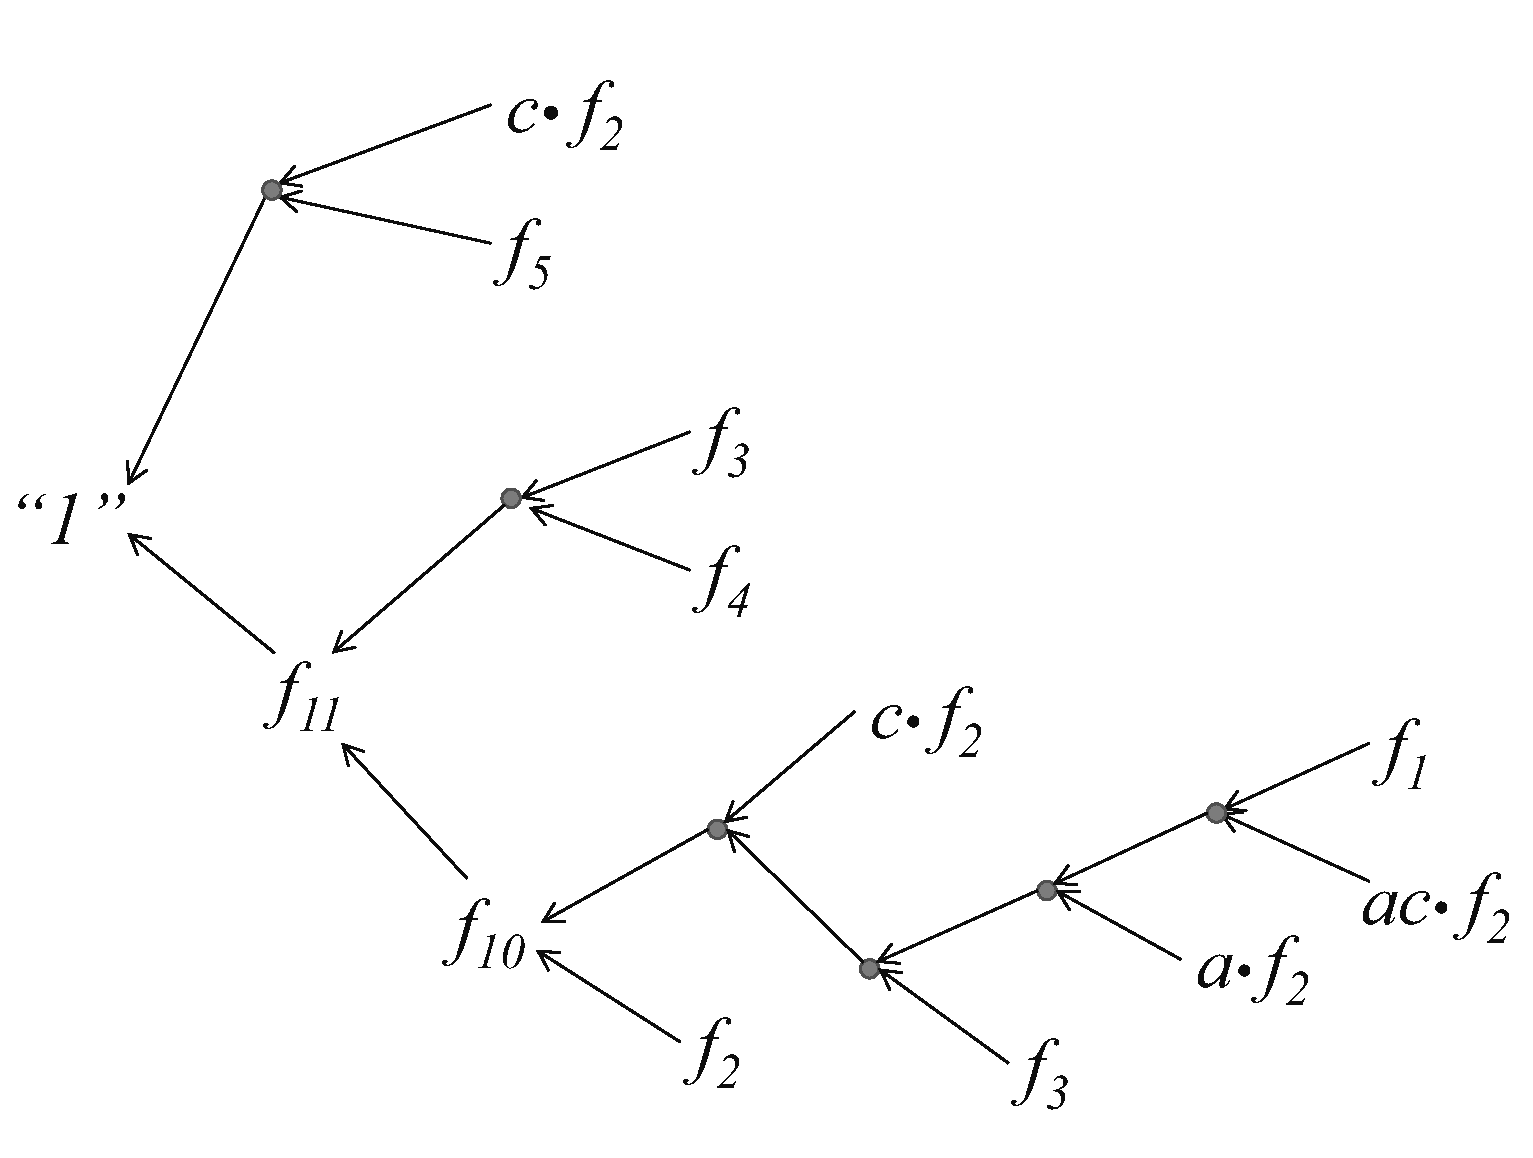
\includegraphics[width=\textwidth]{newfig/refutation_tree.eps}
\caption{Generating refutation trees to record unsat cores}
\label{fig:refute}
\end{figure}

In the figure, the nodes of the graph correspond to the polynomials
utilized in Buchberger's algorithm. The leaf nodes always correspond
to polynomials from the given generating set. An edge $e_{ij}$ from
node $i$ to node $j$ signifies that the polynomial at node $j$ results
from polynomial at node $i$. For example, consider the computation
$Spoly(f_1,f_2)\xrightarrow{F}_+ f_{10}$, where $f_{10} = a + c +
1$. Since $Spoly(f_1, f_2) = f_1 - ac\cdot f_2$, the leaves
corresponding to $f_1$ and $ac\cdot f_2$ are created. The reduction
$Spoly(f_1,f_2)\xrightarrow{F}_+ f_{10}$ is carried out as the
following sequence of 1-step divisions:
$Spoly(f_1,f_2)\xrightarrow{a\cdot f_2} ~\xrightarrow{f_3}~
\xrightarrow{c\cdot f_2}  ~\xrightarrow{f_2} f_{10}$. This is depicted
as the bottom subtree in the figure, terminating at polynomial
$f_{10}$. Moreover, the multiplication $a\cdot f_2$ implies that
division by $f_2$ resulted in the quotient $a$. The refutation tree of
Fig. \ref{fig:refute} shows further that
$Spoly(f_3,f_4)\xrightarrow{f_{10}} f_{11} = c+1$ and, finally,
$Spoly(f_5,f_2)\xrightarrow{f_{11}} 1$. 
 
To identify an $F_c \subset F$, we start from the refutation node
``1'', and traverse the graph in reverse, all the way up to the
leaves. Then, all the leaves in the transitive fanin of ``1''
constitute an unsat core. The polynomials (nodes) that do not lie in
the transitive fanin of ``1'' can be safely discarded from $F_c$. From
Fig. \ref{fig:refute}, $F_c = \{f_1,f_2,f_3,f_4,f_5\}$ is identified
as an unsat core of $F$. 

\section{Reducing the Size of the Infeasible Core $F_c$}
\label{sec:alg}
The core $F_c$ obtained from the aforementioned procedure may
contain redundant elements which could be discarded. For
example, consider the core $F_c=\{f_1,\dots, f_5\}$ generated in the
previous section. While $F_c$ is a smaller infeasible core of $F$, it
is not minimal. In fact, Example 1 shows that $F_{c4} =\{f_1,f_2,f_4,f_5\}$ is the
minimal core, where $F_{c4} \subset F_{c}$. Clearly, the polynomial
$f_3 \in F_c$ is a redundant element of the core and can be 
discarded. We will now describe techniques to further reduce the size
of the unsat core by identifying such redundant elements. 
%how the size of this core could be reduced further.  
For this purpose, we will have to perform a more 
systematic book-keeping of the data generated during the execution of
Buchberger's algorithm and the refutation tree. 

\subsection{Identifying redundant polynomials from the refutation tree}

We record the S-polynomial reduction
$Spoly(f_i,f_j)\xrightarrow{F}_+{g_{ij}}$ that give a non-zero
remainder when divided by the system of polynomials $F$ at that
moment. The remainder $g_{ij}$ is a polynomial combination of
$Spoly(f_i,f_j)$ and the current basis $F$; thus, it can be
represented as:
\begin{equation}
\label{eqn1}
g_{ij}= S(f_i,f_j)+\displaystyle\sum_{k=1}^m c_kf_k,
\end{equation}
where $0\neq c_k\in\mathbb{F}[x_1,\ldots,x_d]$ and
$\{f_1,\ldots,f_m\}$ is the ``current'' system of polynomials
$F$. For each non-zero $g_{ij}$, we will record the following data: 

\begin{equation}
\label{data1}
((g_{ij})(f_{i},h_{ij})(f_{j},h_{ji})| (c_{k1},f_{k1}),(c_{k2},f_{k2}),\dots,(c_{kl},f_{kl}))
\end{equation}

In Eqns. (\ref{eqn1}) and (\ref{data1}), $g_{ij}$ denotes the
remainder of the $S$-polynomial $Spoly(f_i,f_j)$ modulo the current system
of polynomials $f_1,\ldots,f_m$, and we denote by  

$$h_{ij}:=\displaystyle\frac{LCM(lm(f_i),lm(f_j))}{lt(f_i)},
h_{ji}:= - \displaystyle\frac{LCM(lm(f_i),lm(f_j))}{lt(f_j)}$$ 
the coefficients of $f_i$, respectively $f_j$, in the $S$-polynomial
$Spoly(f_i,f_j)$. Furthermore, in Eqn. (\ref{data1}), $(c_{k1}, \dots
c_{kl})$ are the respective quotients of division by
polynomials $(f_{k1},\dots,f_{kl})$, generated during the $Spoly$ reduction.  
%polynomial coefficients of  that appear in the
%division process. 

\begin{Example}
Revisiting Ex. \ref{ex:1}, and Fig. \ref{fig:refute}, the data
corresponding to $Spoly(f_1,f_2)$\\$\xrightarrow{F}_+  g_{12} = f_{10}$
reduction is obtained as the following sequence of computations:
$$f_{10}=g_{12}=f_1-acf_2-af_2-f_3-cf_2-f_2.$$ As the coefficient
field is $\mathbb{F}_2$ in this example, $-1 = +1$, so:
$$f_{10}=g_{12}=f_1+acf_2+af_2+f_3+cf_2+f_2$$ is obtained.
The data is recorded according to Eqn. (\ref{data1}):

\begin{center}
$((f_{10}=g_{12}), (f_1,1)(f_2,ac)|(a,f_2),(1,f_3),(c,f_2),(1,f_2))$
\end{center}

\end{Example}

Our approach and the book-keeping terminates when we obtain ``1'' as the
remainder of some S-polynomial modulo the current system of 
generators. As an output of the Buchberger's algorithm, we can obtain
not only the Gr\"obner basis $G = \{g_1,\ldots,g_t\}$, but also a
matrix $M$ of polynomials such that: 

\vspace{-0.1in}
\begin{center}
\begin{align}
   \begin{bmatrix}
           g_{1} \\
           g_{2} \\
           \vdots \\
           g_{t}
         \end{bmatrix}
    &= M \begin{bmatrix}
           f_{1} \\
           f_{2} \\
           \vdots \\
           f_{s}
         \end{bmatrix}
  \end{align}

\end{center}

Each element $g_i$ of $G$ is a polynomial combination of $\{f_1, \dots,
f_s\}$. Moreover, this matrix $M$ is constructed precisely using the
data that is recorded in the form of Eqn. (\ref{data1}). We now give a condition
when the matrix $M$ may identify some redundant elements. 


\begin{Theorem}
\label{thm}
With the notations above, we have that a core for the system of
generators $F = \{f_1,\dots,f_s\}$ of the ideal $J$ is given by the
union of those $f_i$'s from $F$ that appear in the data recorded above
and correspond to the nonzero entries in the matrix $M$.  
\end{Theorem}

\begin{Proof}
In our case, since the variety is empty, and hence the ideal is
unit, we have that $G = \{g_1=1\}$ and $t=1$. Therefore $M=
[a_1, \ldots, a_s]$ is a vector. Then the output of the algorithm
gives: $1 = a_1f_1+\cdots + a_s f_s.$ Clearly, if $a_i=0$ for some $i$ then
$f_i$ does not appear in this equation and should not be included in
the infeasible core of $F$. 

\end{Proof}


\begin{Example}

Corresponding to Example \ref{ex:1} and the refutation tree shown in
Fig. \ref{fig:refute}, we discover that the polynomial $f_3$ is used
only twice in the division process. In both occasions, the quotient of
the division is 1. From Fig. \ref{fig:refute}, it follows that:
\begin{equation}
1 = (f_2 + f_5) + \dots + \mathbf{1\cdot f_3} + \dots + \mathbf{1\cdot
  f_3}+ \dots + (f_1 + f_2)
\end{equation}

Since $1 + 1 = 0$ over $\F_2$, we have that the entry in $M$
corresponding to $f_3$ is 0, and so $f_3$ can be discarded from the
core. 
\end{Example}

\subsection{The GB-Core Algorithm Outline}

The following steps describe an algorithm (GB-Core) that allows us to compute a
refutation tree of the polynomial set and corresponding matrix $M$. 

{\bf Inputs:} Given a system of polynomials $F=\{f_1,\ldots,f_s\}$, a
monomial order $>$ on $\mathbb{F}[x_1,\ldots,x_d]$.  

{\bf S-polynomial reduction:} We start computing the S-polynomials of the system of
generators $\{f_1,\ldots,f_s\}$, then divide each of them by the
current basis $G=\{f_1,\dots,f_s,\dots,f_m\}$, which is the
intermediate result of Buchberger's algorithm.  
In this way, we obtain expressions of the following type:
\begin{equation}
\label{eqn:red}
g_{ij}= \underbrace{h_{ij}f_{i}+h_{ji}f_{j}}_{Spoly(f_i,f_j)}+\displaystyle\sum_{k=1}^m c_kf_k
\end{equation}
If the remainder $g_{ij}$ is non-zero, we denote it by
$f_{m+1}$ and add it to the current set of generators $G$. We
also record the data as in Eqn. (\ref{data1}): 
\begin{displaymath}
((f_{m+1}=g_{ij})(f_{i},h_{ij})(f_{j},h_{ji})| (c_{k1},f_{k1}),(c_{k2},f_{k2}),\dots,(c_{kl},f_{kl}))
\end{displaymath}
This data forms a part of the refutation tree rooted at node $f_{m+1}$.

{\bf Recording the coefficients:} In Eqn. (\ref{eqn:red}) we obtain a
vector of polynomial coefficients $c_k$ where $k>s$. These
coefficients are associated with new elements (remainders) in the
Gr\"obner basis, that are not a part of the unsat core. 
%which cannot benefit the UNSAT core extraction. 
Since each polynomial $f_k$, ($k>s$) is generated by
$\{f_1,\dots,f_s\}$, we can re-express $f_k$ in terms of $\{f_1,\dots,
f_s\}$. Thus, each $f_k, k>s$ can be written as $f_k = d_1f_1 + \dots
+ d_sf_s$. This process adds a new row $(d_1,\dots,d_s)$ to the
coefficient matrix $M$. 


%% Therefore we need to rewrite the vector to
%% one with only $c_k, k=1\dots s$, which can be achieved by substituting $f_k,k>s$ by $f_1,\dots,f_s$:
%% initially we have $f_{s+1}= c_1f_1 + c_2f_2 + \cdots + (h_{ij}+c_i)f_{i}+\cdots+(h_{ji}+c_j)f_{j}+\cdots+c_sf_s$,
%% inductively if we can present $f_{s+1}$ to $f_{s+k-1}$ by $f_1,\dots,f_s$, we can also rewrite
%% $f_{s+k} = d_1f_1+\cdots+d_sf_s$. Then we add a new row $ (d_1,\dots,d_s ) $ to coefficient matrix $M$.

{\bf Termination and refutation tree construction:} We perform
S-polynomial reductions and record these coefficients  generated
during the division until the remainder $f_m = 1$ is encountered. The
corresponding data is stored in a data-structure $D$ corresponding to
Eqn. (\ref{data1}). The matrix $M$ is also constructed. From this
recorded data the refutation tree can be easily derived. 

%the algorithm
%will generate a set of new generators $G$ and coefficient matrix $M$.
%Meanwhile we can construct the refutation tree with the recorded data.
We start with the refutation node ``$f_m=1$'':
\begin{displaymath}
((f_{m}=1)(f_{i},h_{ij})(f_{j},h_{ji})| (c_{k1},f_{k1}),(c_{k2},f_{k2}),\dots,(c_{kl},f_{kl}))
\end{displaymath}
and recursively substitute the expressions for the polynomials $f_k$
($k>s$) until we obtain the tree with all the leaf nodes corresponding
to the original set of polynomials $\{f_1,\dots,f_s\}$. Algorithm
\ref{algo:gbcore} describes this data recording through which the
refutation tree $T$ and the matrix $M$ is derived. 

\begin{algorithm}[H]
 \caption{GB-core algorithm (based on Buchberger's algorithm)}
 \label{algo:gbcore}
 \begin{algorithmic}[1]

 \REQUIRE $F = \{f_1, \dots, f_s\} \in \F[x_1, \dots, x_d], f_i\neq 0$
 \ENSURE Refutation tree $T$ and coefficients matrix $M$
 \STATE{ {Initialize: list $G \gets F$; Dataset $D\gets \emptyset$; $M\gets s\times s$ unit matrix} }
 \FOR {{ each pair $(f_i,f_j)\in G$  }}
 	\STATE  $f_{sp},(f_{i},h_{ij})(f_{j},h_{ji}) \gets$ Spoly($f_i,f_j$) \COMMENT{$f_{sp}$ is the S-polynomial}
 	\STATE{{ $g_{ij}|(c_{k1},f_{k1}),\dots,(c_{kl},f_{kl}) \gets (f_{sp}\xrightarrow{G}_+  g_{ij})$}}
 	\IF{{ $g_{ij} \neq 0$ }}
 		\STATE {{$G \gets G \cup g_{ij}$}}
 		\STATE {{$D \gets D \cup
                    ((g_{ij})(f_{i},h_{ij})(f_{j},h_{ji})|
                    (c_{k1},f_{k1}),(c_{k2},f_{k2}),\dots,(c_{kl},f_{kl}))$}}
                \STATE{{Update matrix $M$}}
 	\ENDIF
 	\IF {{$g_{ij} = 1$}}
 		\STATE {{Construct $T$ from $D$}}
 		\STATE {{ Return($T,M$) }}
 	\ENDIF
 \ENDFOR
 \end{algorithmic}
 \end{algorithm}


Notice that the core can actually be derived directly from the matrix 
$M$. However, we also construct the refutation tree $T$ as it
facilitates an iterative refinement of the core, which is described
in the next section. 

\section{Iterative Refinement of the Unsat Core}
\label{sec:iter}

As with most other unsat core extractors, our algorithm also cannot
generate a minimal core in one execution. To obtain a smaller core, we
 re-execute our algorithm with the core obtained in the current
iteration. We describe two heuristics that are applied to our
algorithm to increase the likelihood of generating a smaller core in
the next iteration.  

%After eliminating all redundant polynomials, we can call our GB engine
%with the new core. 
An effective heuristic should increase the chances that the refutation
``1'' is composed of fewer polynomials.  In our GB-core algorithm, we
use a strategy to pick critical pairs such that polynomials with
larger indexes get paired {\it later} in the order:

$$(f_1,f_2)\to(f_1,f_3)\to(f_2,f_3)\to(f_1,f_4)\to(f_2,f_4)\to\cdots$$

Moreover, for the reduction process
$Spoly(f_i,f_j)\xrightarrow{F}_+g_{ij}$, we pick divisor polynomials from
$F$ following the increasing order of polynomial indexes. Therefore,
by relabeling the polynomial indexes, we can affect their
chances of being selected in the unsat core. We use two criteria to
to affect the polynomial selection in the unsat core. One corresponds
to the \emph{refutation distance}, whereas the other corresponds to
the {\it frequency} with which a polynomial appears in the refutation
tree.  

\begin{Definition}[Refutation Distance]
Refutation distance of a polynomial $f_i$ in a refutation tree
corresponds to the number of edges on the shortest path from refutation
node ``1'' to any leaf node that represents polynomial $f_i$. 
\end{Definition}

On a given refutation tree, polynomials with shorter refutation
distances are used as divisors in later stages of polynomial
reductions; which implies that they may generally have lower-degree
leading terms. This is because we impose a degree-lexicographic term
order, and successive divisions (term cancellations) reduce the degree
of the remainders. However, what is more desirable is to use these
polynomials with lower-degree leading terms earlier in the reduction,
as they can cancel more terms. This may prohibit other (higher-degree)
polynomials from being present in the unsat core. 


%% So polynomials with lower degree
%% leading terms are more  likely to be used as divisors in later steps
%% of reduction.  
%% In other words, polynomials with shorter refutation
%% distance may have lower-degree leading terms. 
%% If lower degree
%% polynomials are used earlier in the division process, they can cancel
%% more terms, and they will appear in the tree more often --- which may
%% imply that they are a part of the core. 
% %such that the probability that they appear in
%the refutation tree is larger.  

Similarly, the motivation for using the \emph{frequency of occurrence}
of $f_i$ in the refutation tree is as follows: polynomials that appear
frequently in the refutation tree may imply that they have certain
properties (leading terms) that give them a higher likelihood of being
present in the unsat core. 

%make them "favourable" in the unsat core
%selection. For example, their leading terms may contain variables
%that are require them to be included in the minimal core. 

We apply both heuristics: after the first iteration of the GB-core
algorithm, we analyze the refutation tree $T$ and sort the polynomials
in the core by the refutation distance criterion, and use the
frequency criterion as the tie-breaker. The following example
illustrates our heuristic.  


%\vspace{5mm}\\
\begin{Example} 
Consider a set of 6 polynomials over $\F_2$ of an
infeasible instance.
\begin{align*}
f_1: x_1x_3+x_3; & ~~~f_2: x_2 + 1\\
f_3: x_2x_3+x_2; & ~~~f_4: x_2x_3\\
f_5: x_2x_3 + x_2 + x_3 + 1; & ~~~f_6 : x_1x_2x_3 +x_1x_3
\end{align*}

After the first iteration of the GB-core algorithm, the core is
identified as $\{f_1, f_2,f_3,f_4\}$, and we obtain a
refutation tree as shown in Fig.\ref{fig:refine}(a).  
\begin{figure}[hbt]
\centering
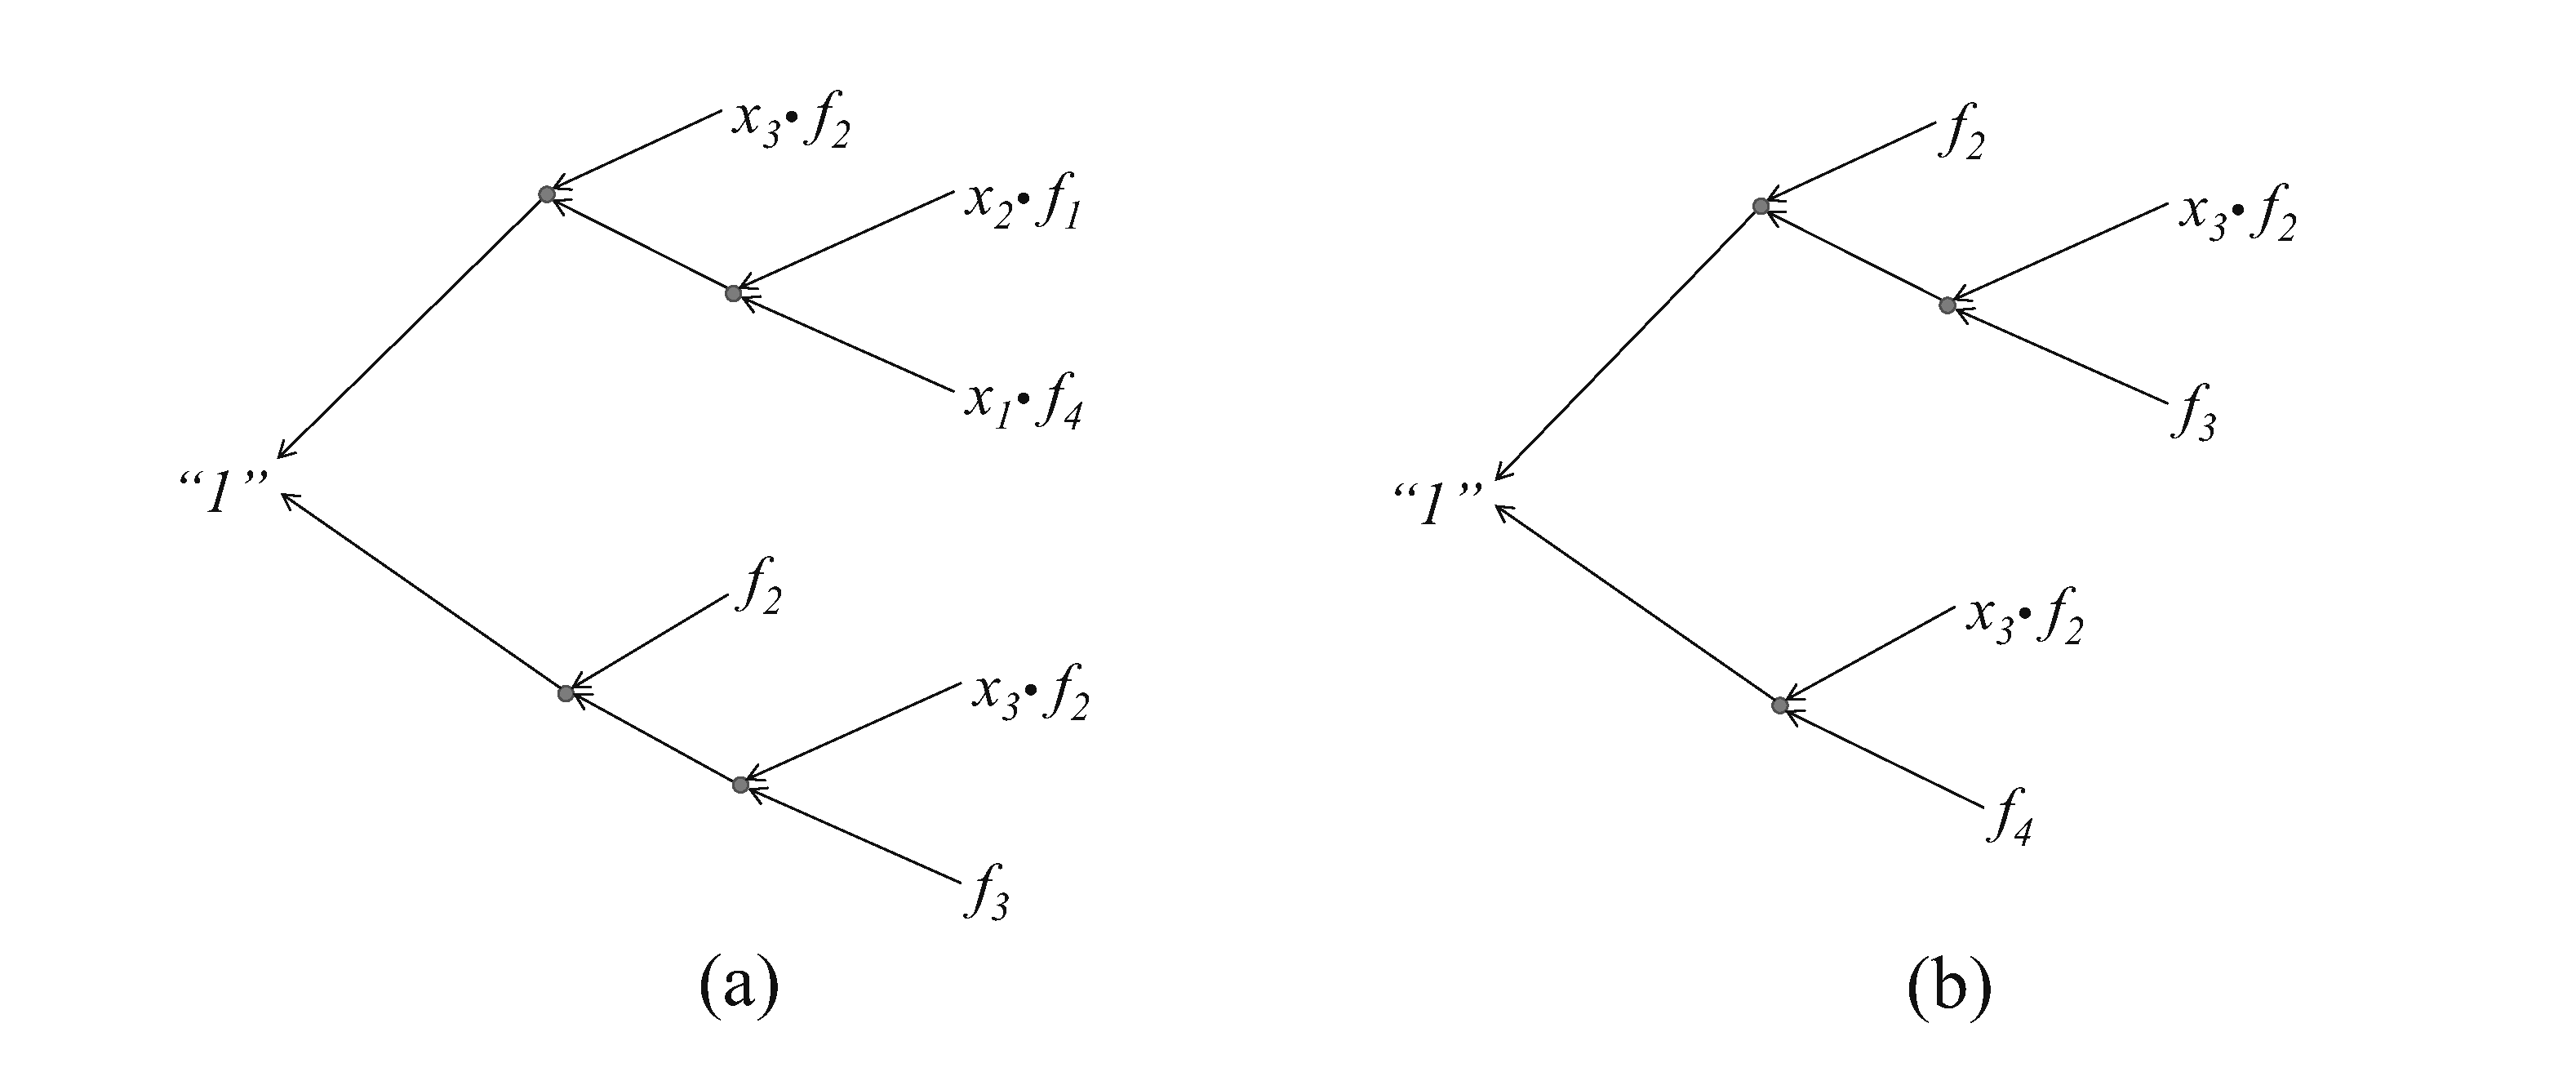
\includegraphics[width=\textwidth]{newfig/core_refine.eps}
\caption{Refutation trees of core refinement example}
\label{fig:refine}
\end{figure}

The refutation distance corresponding to polynomial $f_2$ is equal to
2 levels. Note that while three leaf nodes in Fig. \ref{fig:refine} (a)
correspond to $f_2$, the shortest distance from ``1'' to any $f_2$
node is 2 levels. The refutation distance and frequency measures of
other polynomials are identical -- equal to 3 and 1, respectively --
so their relative ordering is unchanged. We reorder $f_2$ to be the
polynomial with the  smallest index. We re-index the polynomial set 
$f_1'=f_2, f_2' = f_1, f_3' = f_3, f_4' = f_4$
and apply our GB-core algorithm on the core
$\{f_1',f_2',f_3',f_4'\}$. The result is shown in
Fig.\ref{fig:refine}(b) with the core identified as $\{f_1', f_3',
f_4'\} = \{f_2,f_3,f_4\}$. Further iterations do not refine the core
-- i.e. a fix point is reached. 
\end{Example}

\section{Refining the Unsat core using Syzygies}
\label{sec:syz}

%% In some
%% cases our iterative core refining algorithm cannot
%% give us the minimal core when it hits the fixpoint.
%% It indicates the limitation of using re-labelling 
%% strategy, therefore a new method to identify the 
%% redundancy in UNSAT core is needed.

The unsat core obtained through our GB-core algorithm is by nature a
refutation polynomial that equals to 1:  
$$1 = \sum_{i=1}^s c_i\cdot f_i$$
where $0 \neq c_i \in \F[x_1,\dots,x_d]$ and the polynomials
$F = \{f_1,\dots,f_s\}$ form a core. Suppose that a polynomial 
$f_k \in F$ can be represented using a combination of the rest of the
polynomials of the core, e.g.:
$$f_k = \sum_{j\neq k} c_j'f_j.$$

Then we can substitute $f_k$ in terms of the other polynomials in the
refutation. Thus, $f_k$ can be dropped from the core as it is 
redundant. One of the limitations of the GB-core algorithm and the
re-labeling/refinement strategy is that they cannot easily identify
such polynomials $f_k$ in the generating set $F$ that can be composed
of the other polynomials in the basis, i.e. 
$f_k \in \langle F-\{f_k\} \rangle$. We present an approach targeted
to identify such combinations to further refine the core. 
 
 %% Since coefficients $\{c_i\}$ are also polynomials in $\mathbb F[x_1,\dots,x_n]$, we can find 
 %% enormous number of combinations of $\{f_i\}$. Consider finding an algorithmic solution to 
 %% this problem without introducing extra search,
 %% we propose to utilize the \emph{syzygies} generated during
 %% executing the GB-core algorithm.
 
During the execution of Buchberger's algorithm, many critical pairs
$(f_i,f_j)$ do not add any new polynomials in the basis when
$Spoly(f_i,f_j)\xrightarrow{F}_+0$ gives zero remainder. Naturally,
for the purpose of the GB computation, this data is
discarded. However, our objective is to gather more information from
each GB iteration so as to refine the core. Therefore, we further
record the quotient-divisor data from S-polynomial reductions that
result in the remainder 0. Every $Spoly(f_i,f_j)\xrightarrow{F}_+0$
implies that some polynomial combination of $\{f_1,\dots,f_s\}$
vanishes: i.e. $c_1f_1 + c_2f_2 + \dots+c_sf_s=0$, for some
$c_1,\dots,c_s$. These elements ($c_1,\dots,c_s$) form a syzygy on $f_1,\dots,f_s$. 

\begin{Definition}[Syzygy \cite{ideals:book}]
Let $F = \{f_1,\dots,f_s\}$. A syzygy on $f_1,\dots,f_s$ is an
$s$-tuple of polynomials $(c_1,\dots,c_s)\in (\F[x_1,\dots,x_d])^s$
such that $\sum_{i=1}^s c_i\cdot f_i = 0$.
\end{Definition}

For each $Spoly(f_i,f_j)\xrightarrow{F}_+0$ reduction, we record the
information on corresponding syzygies as in Eqn. (\ref{eqn:syz}), also
represented in matrix form in Eqn. (\ref{mat:syzygy}):


\begin{equation} \label{eqn:syz}
%\[
 \begin{cases}
 c_1^1f_1+c_2^1f_2+\cdots+c_s^1f_s = 0\\
 c_1^2f_1+c_2^2f_2+\cdots+c_s^2f_s  = 0\\
 \ \ \ \ \ \  \vdots \\
 c_1^mf_1+c_2^mf_2+\cdots+c_s^mf_s = 0  
 \end{cases}
%\]
\end{equation}

%which can be represented in matrix form as:
\begin{center}
\begin{align}
\label{mat:syzygy}
   \begin{bmatrix}
           c_1^1 & c_2^1 & \cdots & c_s^1 \\
           c_1^2 & c_2^2 & \cdots & c_s^2 \\
           \vdots & \vdots & \ddots & \vdots \\
           c_1^m & c_2^m & \cdots & c_s^m
         \end{bmatrix}
    \begin{bmatrix}
           f_{1} \\
           f_{2} \\
           \vdots \\
           f_{s}
         \end{bmatrix}
         &= 0
  \end{align}

\end{center}


\ \\
 Here $\{f_1,f_2,\dots,f_s\}$ is the given core.
 Take one column of the syzygy matrix (e.g. the set of polynomials in $j$-th column
 $c_j^1, c_j^2, \dots, c_j^m$)  and compute its reduced Gr\"obner
 basis $G_r$. If $G_r = \{1\}$, then it means that there exists some
 polynomial vector  $[r_1,r_2,\dots,r_m]$ such that $1 = r_1c_j^1 +
 r_2c_j^2 + \cdots + r_mc_j^m = \sum_{i=1}^m r_ic_j^i.$ 
 If we multiply each row $i$ in the matrix of Eqn. (\ref{mat:syzygy})
 with $r_i$, and sum up all the rows, we will obtain the
 following equation: 
\vspace{-0.2in}
 \begin{center}
\begin{align}
   \begin{bmatrix}
           \sum_{i=1}^m r_ic_1^i & ~~\cdots & ~~ 1 ~~ & ~~ \cdots ~~ & ~~\sum_{i=1}^m r_ic_s^i
         \end{bmatrix}
    \begin{bmatrix}
           f_{1} \\
           f_{2} \\
           \vdots \\
           f_{s}
         \end{bmatrix}
         &= 0
  \end{align}

\end{center}

This implies that 
 $$\sum_{i=1}^m r_ic_1^if_1 + \cdots + f_j
 +\cdots + \sum_{i=1}^m r_ic_s^if_s = 0,$$
or that $f_j$ is a polynomial combination of
$f_1,\dots,f_s$ (excluding $f_j$). Subsequently, we can deduce that $f_j$ can be
discarded from the core. By repeating this procedure, some redundant
polynomials can be identified and size of unsat core can be reduced
further. 

 \begin{Example}
 Revisiting Example\ref{ex:1}, execute the GB-core algorithm and
 record the syzygies on $f_1,\dots,f_s$ corresponding to the
 S-polynomials that give 0 remainder. The coefficients can be
 represented as entries in matrix shown below. For example, the first
 row in the matrix corresponds to the syzygies generated by
 $Spoly(f_1,f_3)\xrightarrow{F}_+0$.  

\begin{equation}\label{eqn:sm}
% \[
 \begin{blockarray}{cccccccccccc}
  && f_1 & f_2 & f_3 & f_4 & f_5 & f_6 & f_7 & f_8 & f_9 & f_{10} \\
  \begin{block}{cc(cccccccccc)}
  Spoly(f_1,f_3)\ & & 1 & a+c+1 & b+1 &0&0&0&0&0&0&1\\
  Spoly(f_2,f_3)\ & & 0 & ac & b &0&0&0&0&0&0&0\\
  Spoly(f_1,f_4)\ & & 1 & c+1 & 1 &b&0&0&0&0&0&1\\
  Spoly(f_2,f_4)\ & & 0 & ac+a & 0 &b&0&0&0&0&0&0\\
  Spoly(f_1,f_5)\ & & 1 & a+c+1 & 0 &0&a&0&0&0&0&1\\
  \end{block}
  \end{blockarray}
% \]
\end{equation}

Usually, we need to generate extra columns compared to the syzygy
matrix of Eqn. (\ref{mat:syzygy}). In this example, we need to add an
extra column for the coefficient of $f_{10}$. This is because $f_{10}$
is not among the original generating set; however, some S-polynomial
pairs require this new remainder $f_{10}$ as a divisor during
reduction. In order to remove this extra column, we need to turn the
non-zero entries in this column to 0 through standard matrix
manipulations. 

Recall that we record $f_{10}$ in $M$ as a nonzero remainder when
reducing S-polynomial pair $Spoly(f_1,f_2)\xrightarrow{F}_+f_{10}$. We
extract this information from the coefficient matrix $M$:
 $$(1 ~~ac+a+c+1 ~~1 ~~0 ~~0 ~~0 ~~0 ~~0 ~~0 )$$

 It represents $f_{10}$ is a combination of $f_1$ to $f_9$:
 $$f_{10} = f_1 + (ac+a+c+1)f_2 + f_3$$
 It can be written in the same syzygy matrix form (with column
 $f_{10}$ present) as follows:

\begin{equation}\label{sr}%  \[
 \begin{blockarray}{cccccccccccc}
  && f_1 & f_2 & f_3 & f_4 & f_5 & f_6 & f_7 & f_8 & f_9 & f_{10} \\
  \begin{block}{cc(cccccccccc)}
  Spoly(f_1,f_2)& & 1 & ac+a+c+1 & 1 &0&0&0&0&0&0&1\\
  \end{block}
  \end{blockarray}
 \end{equation}

 By adding this row vector (Eqn. (\ref{sr})) to the rows in
 Eqn. (\ref{eqn:sm}) corresponding to the non-zero entries in the
 column for $f_{10}$, we obtain the syzygy matrix only for the
 polynomials in the core:
  \[
 \begin{blockarray}{ccccccccccc}
  && f_1 & f_2 & f_3 & f_4 & f_5 & f_6 & f_7 & f_8 & f_9  \\
  \begin{block}{cc(ccccccccc)}
  Spoly(f_1,f_3)\ & & 0 & ac & b &0&0&0&0&0&0\\
  Spoly(f_2,f_3)\  && 0 & ac & b &0&0&0&0&0&0\\
  Spoly(f_1,f_4)\  && 0 & ac+a & 0 &b&0&0&0&0&0\\
  Spoly(f_2,f_4)\  && 0 & ac+a & 0 &b&0&0&0&0&0\\
  Spoly(f_1,f_5)\  && 0 & ac & 1 &0&a&0&0&0&0\\
  \end{block}
  \end{blockarray}
 \]

 We find out there is a ``1" entry in the $f_3$ column. The last row
 implies that $f_3$ is a combination of $f_2, f_5$ ($f_3 = ac f_2 + a
 f_5$), so $f_3$ can be discarded from the core. 

 \end{Example}

The syzygy heuristic gathers extra information from the GB
computation, it is still not sufficient to derive all polynomial
dependencies. In Buchberger's algorithm,  many S-polynomials reduce to
zero, so the number of rows of the syzygy matrix can be much larger than
the size of original generating set. Full GB computation on each
column of the syzygy matrix can become prohibitive to apply
iteratively. For this reason, we only apply the syzygy heuristic
on the smaller reduced core given by our iterative refinement algorithm.

\textbf{Our Overall Approach for Unsat Core Extraction:} i) Given
the set $F = \{f_1,\dots,f_s\}$, we apply the GB-core algorithm,
record the data $D, M$ (Section 4) and the syzygies $S$ on
$f_1,\dots,f_s$. ii) From $M$, we obtain a core $F_c \subseteq
F$. iii) Iteratively refine $F_c$ (Section 5) until $|F_c|$ cannot be
reduced further. iv) Apply the syzygy-heuristic (Section 6) to
identify if some $f_k \in F_c$ is a combination of other polynomials
in $F_c$; all such $f_k$ are discarded from $F_c$. This gives us the
final unsat core $F_c$. 

\section{Experiment results}
\label{sec:exp}


We have implemented our core extraction approach (the GB-Core
and the refinement algorithms) using the \textsc{Singular} symbolic
algebra computation system [v. 3-1-6] \cite{DGPS}. With our
tool implementation, we have performed experiments to extract a
minimal unsat core from a given set of  
polynomials. Our experiments run on a desktop with
3.5GHz Intel $\text{Core}^\text{TM}$ i7-4770K Quad-core CPU, 16 GB RAM and
64-bit Ubuntu Linux OS. The experiments are shown in Table \ref{tab:result}. 

%Nowadays most SAT benchmarks are huge, which choke our GB engine. 
Gr\"obner basis is not an efficient engine for solving contemporary
industry-size CNF-SAT benchmarks, as the translation from CNF introduces
too many variables and clauses for GB engines to handle. In order to
validate our approach, we use a somewhat customized  benchmark
library: i) "aim-100" is a modified version  of the random 3-SAT
benchmark "aim-50/100", modified by adding some redundant clauses; ii)
The "subset" series are generated for random subset sum problems; iii)
"cocktail" is similarly revised from a combination of factorization
and a random 3-SAT benchmark; iv) and "phole4/5" are generated by
adding redundant clauses to pigeon hole benchmarks; v) Moreover,
SMPO and RH benchmarks correspond to hardware equivalence checking
instances of sequential Galois field normal basis modulo multiplier
circuits \cite{SMPO,RHmulti}, compared against a golden model
{\it spec}. Similarly, the "MasVMon" benchmarks are the equivalence
checking  circuits corresponding to Mastrovito multipliers compared
against  Montgomery multipliers \cite{lv:tcad2013}. Some of these are
available as CNF formulae, whereas others were available directly as
polynomials over finite fields. The CNF formulae are translated as
polynomial constraints over $\mathbb{F}_2$ (as shown in
\cite{condrat-tacas07}), and the GB-Core algorithm and the refinement
approach is applied.   
%These benchmarks are in moderate size for our GB engine but not too trivial. 

%\vspace{-0.1in}
\begin{table}[htb]
\centering
\caption{Results of running benchmarks using our tool. 
\small{Asterisk($^*$) denotes that the benchmark was not translated from CNF.} 
Our tool is composed by 3 parts: part I runs a single GB-core algorithm,
part II applies the iterative refinement heuristic to run the GB-core algorithm
iteratively, part III applies the syzygy heuristic.}
{\small 
\begin{tabular}{|c||c|c|c|c|c|c|c|c|c|c|}
\hline
\multirow{3}{2.2cm}{\centering Benchmark} 
& \multirow{3}{0.9cm}{\centering \# Polys} 
& \multirow{3}{0.8cm}{\centering \# MUS} 
& \multicolumn{3}{c|}{\multirow{2}{1.8cm}{\centering Size of core}}
 & \multirow{3}{1.6cm}{\centering \# GB-core iterations}
 & \multicolumn{3}{c|}{\multirow{2}{2.0cm}{\centering Runtime (sec)}}
 & \multirow{3}{1.8cm}{\centering Runtime of PicoMUS (sec)} \\
  & & &\multicolumn{3}{c|}{}& &\multicolumn{3}{c|}{}& \\
  \cline{4-6} \cline{8-10}
    & & & I & II & III & & I & II & III & \\
\hline
\hline
$5\times 5$ SMPO & 240  & 137  & 169 & 137 & 137  & 8  & 1222 & 1938 & 1698 & $<0.1$\\
$4\times 4$ SMPO$^*$ & 84  & 21  & 21 & 21 & 21 & 1  & 125 & 0.3 & 29  & - \\
$3\times 3$ SMPO$^*$ & 45  & 15  & 15 & 15 & 15  & 1  & 6.6 & 0.2 & 5.7 & - \\
$3 \times 3$ SMPO & 17 & 2 & 2 &2 & 2 & 1 & 0.07 & 0.01 & 0.01  & $<0.1$  \\
$4 \times 4$ MasVMont$^*$ & 148 & 83 & 83 & 83 & 83 & 1 & 23 & 139 & 12 & - \\
$3 \times 3$ MasVMont$^*$ & 84 & 53 & 53 & 53 & 53  & 1 & 4.3 & 4.6 & 0.9  & - \\
$2 \times 2$ MasVMont & 27 & 23 & 24 & 23 & 23 & 2 & 1.3 & 1.0 & 80  & $<0.1$ \\
$5\times 5$ RH$^*$ & 142  & 34  & 48 & 35 & 35  & 4  & 997 & 1.0 & 80 & - \\
$4\times 4$ RH$^*$ & 104  & 35  & 43 & 36 & 36  & 3  & 96 & 5.7 & 0.6 & -\\
$3\times 3$ RH$^*$ & 50  & 20  & 20 & 20 & 20  & 1  &2.9 & 3.5 & 10  & -\\
aim-100 & 79 & 22 & 22 & 22 & 22 & 1  & 43 & 0.7 & 0.2 & $<0.1$\\
cocktail & 135 & 4 & 6 & 4 & 4 & 2 & 51 & 0.01 & 0.01  & $<0.1$ \\
subset-1 & 100 & 6 & 6 & 6 & 6 & 1 & 2.4 & 0.01 & 0.01 & $<0.1$ \\
subset-2 & 141 & 19 & 37 & 23 & 21 & 2 & 12 & 1.6 & 1.1 & $<0.1$  \\
subset-3 & 118 & 16 & 13 & 12 & 11 & 2 & 8.6 & 0.2 & 0.07 & $<0.1$ \\
phole4 & 104 & 10 & 16 & 16 & 10 & 1 & 4.3 & 0.2 & 0.5 &  $<0.1$\\
phole5 & 169 & 19 & 30 & 25 & 19 & 3 & 12 & 3.2 & 2.7 & $<0.1$ \\
\hline
\end{tabular}
}
\label{tab:result}  
\end{table} 

In Table \ref{tab:result}, 
%we list the details of our experimental results. In the table, 
\#Polys denotes the given number of polynomials
from which a core is to be extracted. \#MUS is the {\it minimal} core either
extracted by PicoMUS (for CNF benchmarks) or exhaustive deletion method (for non-CNF bencmarks).
 \#GB-core iterations corresponds to the
number of calls to the GB-core engine to arrive at the reduced unsat
core. The second last column shows the improvement in the minimal core
size by applying the syzygy heuristic on those cases which cannot be
iteratively refined further. 
We choose PicoMUS as a comparison to our tool because it is a state-of-art MUS extractor,
and the results it returned for our set of benchmarks are proved to be minimal. 
The data shows that in most of these
cases, our tool can produce a minimal core. For the subset-3
benchmark, we obtain another core with even smaller size than the one from PicoMUS. The results
demonstrate the power of the Gr\"obner basis technique to identify the
causes of unsatisfiability. 
%From the
%experimental results we can also make the observation that the GB-core
%algorithm, particularly Theorem \ref{thm}, offers quite a lot of scope for identifying redundant
%polynomials that can be eliminated from the core --- without resorting
%to a brute-force membership check of every polynomial $f_i \in F -
%\{f_i\}$. 



\section{Conclusions}\label{sec:conc}
This paper addresses the problem of identifying an infeasible core of
a set of multivariate polynomials, with coefficients from a field,
that have no common zeros. The problem is posed in the context of
computational algebraic geometry and solved using the Gr\"obner basis
algorithm. We show that by recording the data produced by the
Buchberger's algorithm -- the $Spoly(f_i,f_j)$ pairs, as well as the
polynomials of $F$ used in the division process
$Spoly(f_i,f_j)\xrightarrow{F}_+ 1$ -- we can identify certain
conditions under which a polynomial can be discarded from a core. An
algorithm was implemented within the Singular computer algebra tool
and some experiments were conducted to validate the approach. While
the use of GB engines for SAT solving has a rich history, the problem
of unsat core identification using GB-engines has not been addressed
by the SAT community. We hope that this paper will kindle some
interest in this topic which is worthy of attention from the SAT
community -- particularly when there seems to be a renewal of interest
in the use of Gr\"obner bases for formal verification
\cite{lv:tcad2013,gao:qe-gf-gb,kalla:fmcad_tut2015,rolf:date16}.    
